% +------------------------------------------------------------------------+
% | Reference manual page: Regular_triangulation_3.tex
% +------------------------------------------------------------------------+
% | 27.3.2000   Monique Teillaud
% | Package: Triangulation3
% | 
\RCSdef{\RCSRegulartriangulationRev}{$Id$}
\RCSdefDate{\RCSRegulartriangulationDate}{$Date$}
% |
%%RefPage: end of header, begin of main body
% +------------------------------------------------------------------------+


\begin{ccRefClass}{Regular_triangulation_3<RegularTriangulationTraits_3,TriangulationDataStructure_3>}

\ccDefinition
  Let ${S}^{(w)}$ be a set of weighted points in $\R^3$. Let
${p}^{(w)}=(p,w_p), p\in\R^3, w_p\in\R$ and 
${z}^{(w)}=(z,w_z), z\in\R^3, w_z\in\R$ be two weighted points. 
A weighted point
${p}^{(w)}=(p,w_p)$ can also be seen as a sphere of center $p$ and
radius $\sqrt{w_p}$. 
The \textit{power product} (or  \textit{power distance} ) 
between ${p}^{(w)}$ and ${z}^{(w)}$ is
defined as 
\[\Pi({p}^{(w)},{z}^{(w)}) = {\|{p-z}\|^2-w_p-w_z}\]
where $\|{p-z}\|$ is the Euclidean distance between $p$ and $z$. 
 ${p}^{(w)}$ and ${z}^{(w)}$
are said to be \textit{orthogonal} if $\Pi{({p}^{(w)}-{z}^{(w)})}
= 0$ (see Figure~\ref{Triangulation3-fig-ortho}).

Four weighted points have a unique common orthogonal weighted point called
the \textit{power sphere}. A sphere ${z}^{(w)}$ is said to be
\textit{regular} if $\forall {p}^{(w)}\in{S}^{(w)},
\Pi{({p}^{(w)}-{z}^{(w)})}\geq 0$.

A triangulation of ${S}^{(w)}$ is \textit{regular} if the power spheres
of all simplices are regular. 

\ccInclude{CGAL/Regular_triangulation_3.h}

\ccParameters

The first template argument must be a model of the
\ccc{RegularTriangulationTraits_3} concept.

The second template argument must be a model of the
\ccc{TriangulationDataStructure_3} concept.
It has the default value \ccc{Triangulation_data_structure_3<Triangulation_vertex_base_3<RegularTriangulationTraits_3>, Regular_triangulation_cell_base_3<RegularTriangulationTraits_3> >}.


\ccInheritsFrom{\ccc{Triangulation_3<RegularTriangulationTraits_3,TriangulationDataStructure_3>}}

\ccTypes
\ccThree{typedef RegularTriangulationTraits_3::Weighted_point_3}{Weighted_point}{}

\ccTypedef{typedef RegularTriangulationTraits_3::Bare_point Bare_point;}
{The type for points
\ccc{p} of weighted points ${p}^{(w)}=(p,w_p)$}
\ccGlue
\ccTypedef{typedef RegularTriangulationTraits_3::Weighted_point_3 Weighted_point;}{}

\ccCreation
\ccCreationVariable{rt}


\ccThree{Regular_triangulation_3<RegularTriangulationTraits_3,TriangulationDataStructure_3>}
{rt( RegularTriangulationTraits_3 traits );xxx}{}

\ccConstructor{Regular_triangulation_3
(const RegularTriangulationTraits_3 & traits = RegularTriangulationTraits_3())}
{Creates an empty regular triangulation, possibly specifying a traits class
\ccc{traits}.}

\ccConstructor{Regular_triangulation_3
(const Regular_triangulation_3 & rt1)} {Copy constructor.}

\ccConstructor{template < class InputIterator >
       Regular_triangulation_3 (InputIterator first, InputIterator last,
 const RegularTriangulationTraits_3& traits = RegularTriangulationTraits_3())}
{Equivalent to constructing an empty triangulation with the optional 
traits class argument and calling \ccc{insert(first,last)}.}

\ccOperations


\ccHeading{Insertion}
\ccThree{OutputIterator}{dt.insertxx}{}

The following methods, which already exist in \ccc{Triangulation_3}, are
overloaded to ensure the property that all power spheres are regular.

\ccMethod{Vertex_handle insert(const Weighted_point & p,
                               Cell_handle start = Cell_handle() );}
{Inserts weighted point \ccc{p} in the triangulation. The optional 
argument \ccc{start} is used as a starting place for the search.\\
If this insertion creates a vertex, this vertex is returned.\\
If \ccc{p} coincides with an existing vertex and has a greater weight, 
then the existing weighted point becomes hidden (see 
\ccc{RegularTriangulationCellBase_3}) and \ccc{p} replaces it as vertex 
of the triangulation.\\
If \ccc{p} coincides with an already existing vertex (both point and 
weights being equal), then this vertex is returned and the triangulation 
remains unchanged.\\
Otherwise if \ccc{p} does not appear as a vertex of the triangulation, 
then it is stored as a hidden point and this method returns the default 
constructed handle.}

\ccMethod{Vertex_handle insert(const Weighted_point & p, Vertex_handle hint);}
{ Same as above but uses \ccc{hint} as a starting place for the search. }

\ccMethod{Vertex_handle insert(const Weighted_point & p, Locate_type lt,
                               Cell_handle loc, int li, int lj);}
{Inserts weighted point \ccc{p} in the triangulation and returns the corresponding
 vertex. Similar to the above \ccc{insert()} function, but takes as additional
 parameter the return values of a previous location query.  See description of
 \ccc{Triangulation_3::locate()}.}

The following method allows one to insert several points.

\ccMethod{template < class InputIterator >
          std::ptrdiff_t
          insert(InputIterator first, InputIterator last);}
{Inserts the weighted points in the range $\left[\right.$\ccc{first},
\ccc{last}$\left.\right)$. 
Note that this function is not guaranteed to insert the points
following the order of \ccc{InputIterator}.
It returns the difference of the number of vertices between after and
before the insertions (it may be negative due to hidden points).
\ccPrecond{The \ccc{value_type} of \ccc{first} and \ccc{last} is
\ccc{Weighted_point}.}}

The following methods, which already exist in \ccc{Triangulation_3}, are
overloaded to ensure that hidden points are well created and maintained.

\ccMethod{template <class CellIt>
     Vertex_handle insert_in_hole(Weighted_point p, CellIt cell_begin, CellIt cell_end,
	                          Cell_handle begin, int i);}
{Creates a new vertex by starring a hole.  It takes an iterator range
[\ccc{cell_begin}; \ccc{cell_end}[ of \ccc{Cell_handle}s which specifies
a hole: a set of connected cells (resp. facets in dimension 2) which is
star-shaped wrt \ccc{p}.
(\ccc{begin}, \ccc{i}) is a facet (resp. an edge) on the boundary of the hole,
that is, \ccc{begin} belongs to the set of cells (resp.  facets) previously
described, and \ccc{begin->neighbor(i)} does not.  Then this function deletes
all the cells (resp. facets) describing the hole, creates a new vertex
\ccc{v}, and for each facet (resp. edge) on the boundary of the hole, creates
a new cell (resp. facet) with \ccc{v} as vertex.  Then \ccc{v->set_point(p)}
is called and \ccc{v} is returned.\\
If the hole contains interior vertices, each of them is hidden by the insertion
of \ccc{p} and is stored in the new cell which contains it.
\ccPrecond{\ccVar.\ccc{dimension()} $\geq 2$, the set of cells (resp. facets in
dimension 2) is connected, not empty, its boundary is connected, and \ccc{p}
lies inside the hole, which is star-shaped wrt \ccc{p}}.}

\ccMethod{template <class CellIt>
     Vertex_handle insert_in_hole(Weighted_point p, CellIt cell_begin, CellIt cell_end,
	                          Cell_handle begin, int i, Vertex_handle newv);}
{ Same as above, except that \ccc{newv} will be used as the new vertex, which
  must have been allocated previously with e.g. \ccc{create_vertex}.}


\ccHeading{Removal}

\ccMethod{void remove(Vertex_handle v);}
{Removes the vertex \ccc{v} from the triangulation.}

\ccHeading{Queries}
\ccThree{OutputIterator}{rt.side of powerxx}{}

Let us remark that 
\[\Pi({p}^{(w)}-{z}^{(w)}) > 0\]
is equivalent to\\
\centerline{\ccc{p} lies outside the sphere with center \ccc{z} and radius
$\sqrt{w_p^2+w_z^2}$.}\\
This remark helps provide an intuition about the following predicates.

\begin{figure}[htbp]
\begin{ccTexOnly}
\begin{center} 
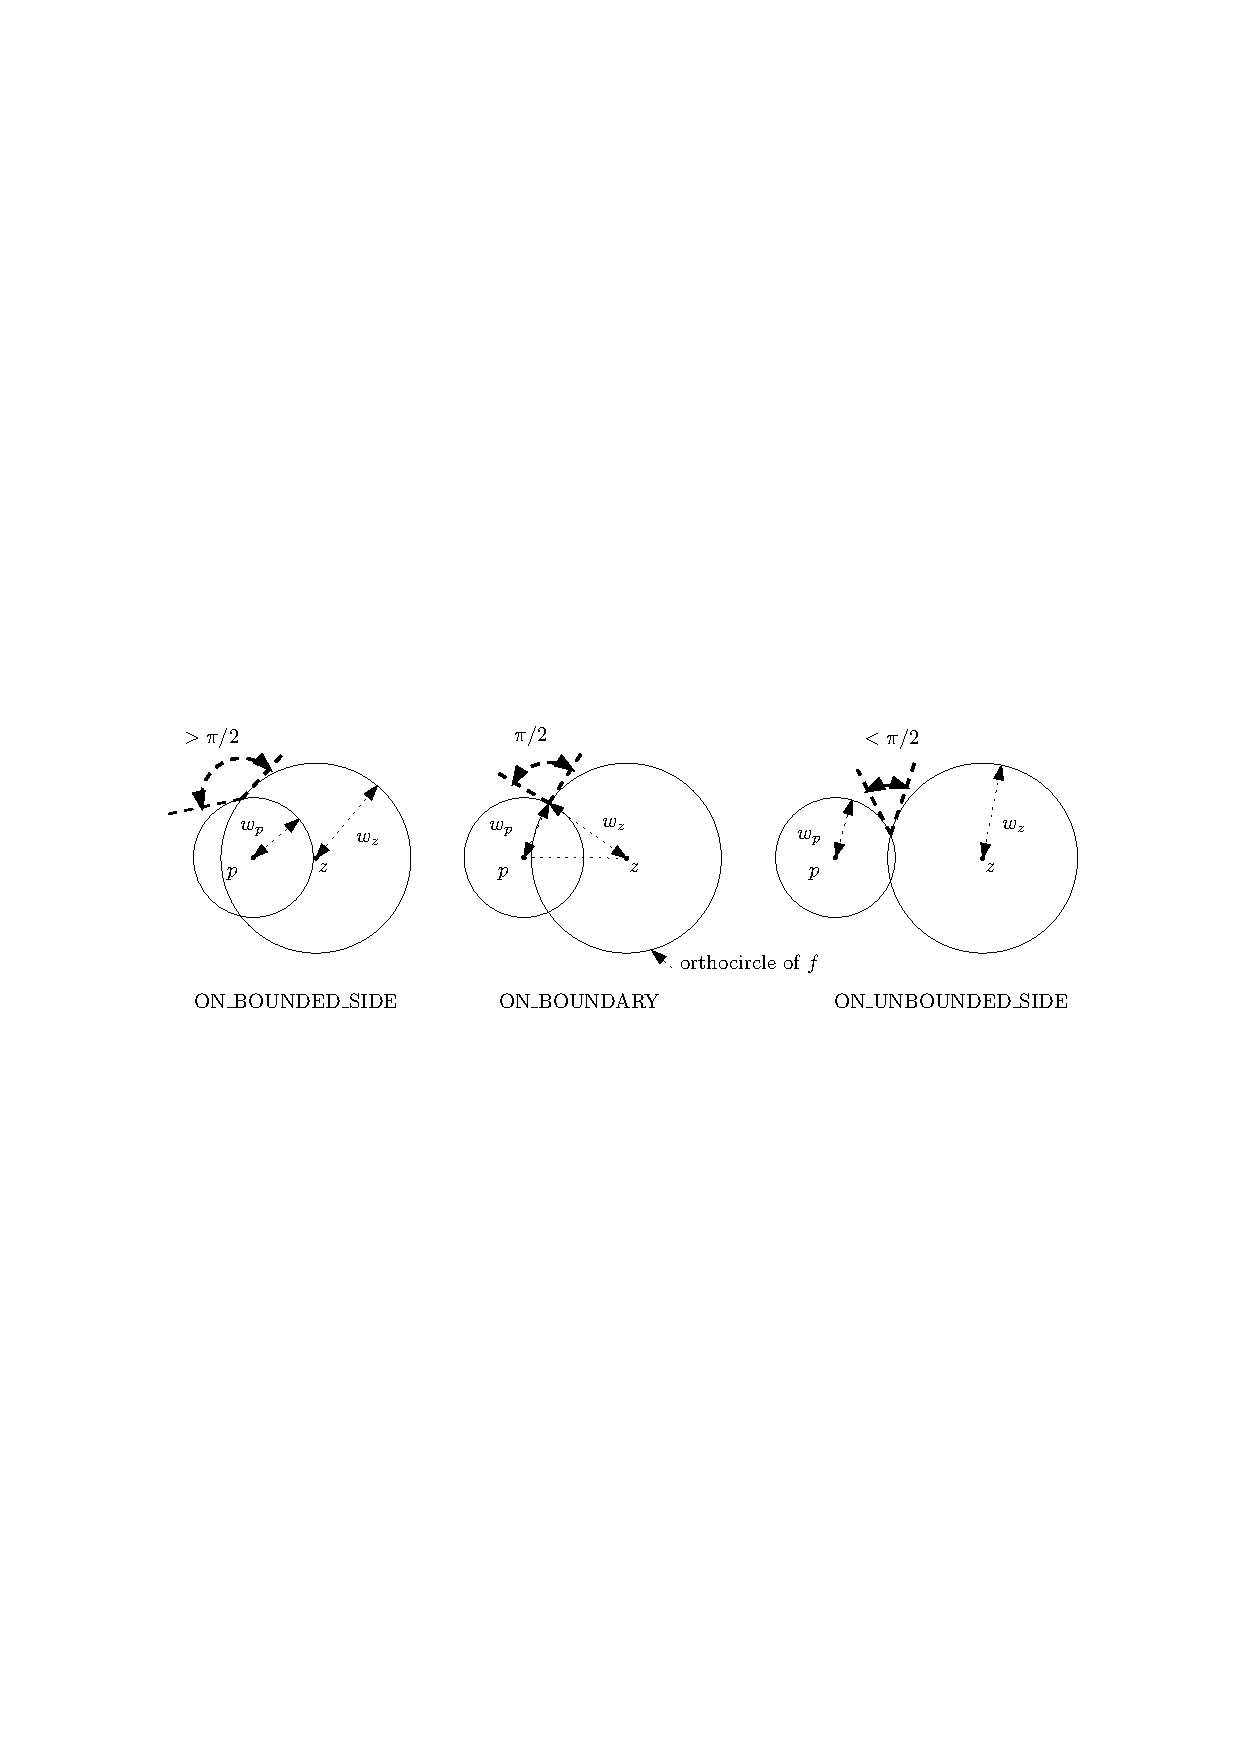
\includegraphics{Triangulation_3_ref/sidedim2} 
\end{center}
\end{ccTexOnly}
\caption{side\_of\_power\_circle.
\label{Triangulation3-fig-sidedim2}}
\begin{ccHtmlOnly}
<CENTER>
<img border=0 src="./sidedim2.gif" align=middle alt="side_of_power_circle"> 
</CENTER>
\end{ccHtmlOnly}
\end{figure} 

\ccMethod{Bounded_side
          side_of_power_sphere(Cell_handle c, const Weighted_point & p) const;}
{Returns the position of the weighted point $p$ with respect to the
power sphere of \ccc{c}. More precisely, it returns:\\
- \ccc{ON_BOUNDED_SIDE} if $\Pi({p}^{(w)}-{z(c)}^{(w)})<0$ where
${z(c)}^{(w)}$ is the power sphere of \ccc{c}. For an
infinite cell this means either that \ccc{p} lies strictly in the half
space limited by its finite facet and not containing any other point
of the triangulation, or that the angle 
between \ccc{p} and the power circle of the \textit{finite} facet of \ccc{c}
is greater than $\pi/2$. \\  
- \ccc{ON_BOUNDARY} if p is orthogonal to the power sphere of \ccc{c}
i.e. $\Pi({p}^{(w)}-{z(c)}^{(w)})=0$. For an infinite cell this means
that \ccc{p} is orthogonal to the power circle of its \textit{finite} facet.\\ 
- \ccc{ON_UNBOUNDED_SIDE} if $\Pi({p}^{(w)}-{z(c)}^{(w)})>0$
i.e. the angle between the weighted point \ccc{p} and the power sphere
of \ccc{c} is less than $\pi/2$ or if these two spheres do not
intersect. For an 
infinite cell this means that \ccc{p} does not satisfy either of the
two previous conditions. 
\ccPrecond{\ccVar.\ccc{dimension()} $=3$.}}

\ccMethod{Bounded_side
	  side_of_power_circle(const Facet & f, 
			const Weighted_point & p) const;}
{Returns the position of the point \ccc{p} with respect to the
power circle of \ccc{f}. More precisely, it returns:\\
--- in dimension~3:\\
-- For a finite facet,\\
\ccc{ON_BOUNDARY} if \ccc{p} is orthogonal to the power circle in the
plane of the facet,\\ 
\ccc{ON_UNBOUNDED_SIDE} when their angle is less than $\pi/2$,\\
\ccc{ON_BOUNDED_SIDE} when it is greater than $\pi/2$ (see
Figure~\ref{Triangulation3-fig-sidedim2}).\\ 
-- For an infinite facet, it considers the plane defined by the finite
facet of the cell \ccc{f.first}, and does the same as in
dimension~2 in this plane.\\
--- in dimension~2:\\
-- For a finite facet,\\
\ccc{ON_BOUNDARY} if \ccc{p} is orthogonal to the circle,\\
\ccc{ON_UNBOUNDED_SIDE} when the angle between \ccc{p} and the
power circle of \ccc{f} is less than $\pi/2$,
\ccc{ON_BOUNDED_SIDE} when it is greater than $\pi/2$.\\ 
-- For an infinite facet,\\
\ccc{ON_BOUNDED_SIDE} for a point in the open half plane defined by
\ccc{f} and not containing any other point of the triangulation,\\
\ccc{ON_UNBOUNDED_SIDE} in the other open half plane.\\
If the point \ccc{p} is collinear with the finite edge \ccc{e} of
\ccc{f}, it returns:\\
\ccc{ON_BOUNDED_SIDE} if $\Pi({p}^{(w)}-{z(e)}^{(w)})<0$, where
${z(e)}^{(w)}$ is the power segment of \ccc{e} in the line supporting
\ccc{e},\\ 
\ccc{ON_BOUNDARY} if $\Pi({p}^{(w)}-{z(e)}^{(w)})=0$,\\
\ccc{ON_UNBOUNDED_SIDE} if $\Pi({p}^{(w)}-{z(e)}^{(w)})>0$ .
\ccPrecond{\ccVar.\ccc{dimension()} $\geq 2$.}}

\ccMethod{Bounded_side
	  side_of_power_circle(Cell_handle c, int i, 
			const Weighted_point & p) const;}
{Same as the previous method for facet \ccc{i} of cell \ccc{c}.}

\ccMethod{Bounded_side
	  side_of_power_segment(Cell_handle c, const Weighted_point & p)
const;}
{In dimension~1, returns\\
\ccc{ON_BOUNDED_SIDE} if $\Pi({p}^{(w)}-{z(c)}^{(w)})<0$, where
${z(c)}^{(w)}$ is the power segment of the edge represented by
\ccc{c},\\
\ccc{ON_BOUNDARY} if $\Pi({p}^{(w)}-{z(c)}^{(w)})=0$,\\
\ccc{ON_UNBOUNDED_SIDE} if $\Pi({p}^{(w)}-{z(c)}^{(w)})>0$ .
\ccPrecond{\ccVar.\ccc{dimension()} $= 1$.}}

\ccMethod{Vertex_handle nearest_power_vertex(Weighted_point p,
                                       Cell_handle c = Cell_handle());}
{Returns the vertex of the triangulation which is nearest to $p$
with respect to the power distance. This  means that the power
of the  query point \ccc{p} with respect to the weighted point in
the returned vertex is smaller than the power of \ccc{p}
 with respect to the weighted point
in any other vertex. Ties are broken arbitrarily.
The default constructed
handle is returned if the triangulation is empty. 
The optional argument \ccc{c} is a hint
specifying where to start the search.
\ccPrecond{\ccc{c} is a cell of \ccVar.}
} 


\ccMethod{Vertex_handle nearest_power_vertex_in_cell(Weighted_point p,
                                       Cell_handle c);}
{Returns the vertex of the cell \ccc{c} 
that is nearest to $p$
with respect to the power distance.
}

A  weighted point \ccc{p} is said to be in conflict 
with a cell \ccc{c} in dimension 3
(resp. with a facet \ccc{f} in dimension 2) 
if it has a negative power distance 
to the power sphere  of  \ccc{c} 
(resp.  to the power circle of \ccc{f}).
The set of cells (resp. facets in dimension 2) which are in conflict with
\ccc{p} is connected.

\ccMethod{template <class OutputIteratorBoundaryFacets,
                    class OutputIteratorCells,
                    class OutputIteratorInternalFacets>
  Triple<OutputIteratorBoundaryFacets,
         OutputIteratorCells,
         OutputIteratorInternalFacets>
  find_conflicts(const Weighted_point p, Cell_handle c,
                 OutputIteratorBoundaryFacets bfit,
                 OutputIteratorCells cit,
                 OutputIteratorInternalFacets ifit);}
{ Compute the conflicts with \ccc{p}.
 The starting cell
(resp.  facet) \ccc{c} must be in conflict with  \ccc{p}.  
Then this function returns
respectively in the output iterators:\\
-- \ccc{cit}: the cells (resp. facets) in conflict  with  \ccc{p}.\\
-- \ccc{bfit}: the facets (resp. edges) on the boundary of the
conflict  zone, that is, the facets
(resp. edges) \ccc{(t, i)} where the cell (resp. facet) \ccc{t} is in
conflict, but \ccc{t->neighbor(i)} is not.\\
-- \ccc{ifit}: the facets (resp. edges) inside the conflict zone, 
that facets incident to two cells (resp facets) in conflict.\\
Returns the \ccc{Triple} composed of the resulting output iterators.
\ccPrecond{\ccVar.\ccc{dimension()} $\geq 2$, and \ccc{c} is in conflict
with \ccc{p}.}
}

\begin{ccDeprecated}
\ccMethod{template <class OutputIterator>
  OutputIterator
  vertices_in_conflict(Weighted_point p, Cell_handle c,
                       OutputIterator res);}
{This function is renamed \ccc{vertices_on_conflict_zone_boundary} since CGAL-3.8.}
\end{ccDeprecated}
\ccMethod{template <class OutputIterator>
  OutputIterator
  vertices_on_conflict_zone_boundary(Weighted_point p, Cell_handle c,
                                     OutputIterator res);}
{Similar to \ccc{find_conflicts()}, but reports the vertices which are on the
boundary of the conflict zone of \ccc{p}, in the output iterator \ccc{res}.
Returns the resulting output iterator.
\ccPrecond{\ccVar.\ccc{dimension()} $\geq 2$, and \ccc{c} is a cell containing
 \ccc{p}.}
}

\ccMethod{template <class OutputIterator>
  OutputIterator
  vertices_inside_conflict_zone(Weighted_point p, Cell_handle c,
                                OutputIterator res);}
{Similar to \ccc{find_conflicts()}, but reports the vertices which are in
  the interior of the conflict zone of \ccc{p}, in the output iterator
  \ccc{res}. The vertices that are on the boundary of the conflict zone are
  not reported.
Returns the resulting output iterator.
\ccPrecond{\ccVar.\ccc{dimension()} $\geq 2$, and \ccc{c} is a cell containing
 \ccc{p}.}
}

In the weighted setting, a face (cell, facet, edge or vertex) 
is said to be a Gabriel face iff
the  smallest sphere  orthogonal to the weighted 
points associated to its vertices,
has a positive power product with the weighted point
of any other vertex of the triangulation.
Any weighted Gabriel face belongs to the
regular triangulation, but the reciprocal is not true.
The following member functions test the Gabriel property of the
faces of the regular triangulation.
\ccMethod{bool is_Gabriel(Cell_handle c, int i);}{}
\ccGlue 
\ccMethod{bool is_Gabriel(Cell_handle c, int i, int j);}{}
\ccGlue 
\ccMethod{bool is_Gabriel(const Facet& f);}{}
\ccGlue
\ccMethod{bool is_Gabriel(const Edge& e);} {}
\ccGlue
\ccMethod{bool is_Gabriel(Vertex_handle v);}{}


\ccHeading{Power diagram}
\ccIndexMainItem{Power diagram}
\cgal\ offers several functionalities to display the Power diagram of 
a set of points in 3D.

Note that the user should use a kernel with exact constructions in order
to guarantee the computation of the Voronoi diagram (as opposed to computing
the triangulation only, which requires only exact predicates).

\ccMethod{Weighted_point dual(Cell_handle c) const;}
{Returns the weighted circumcenter of the four vertices of c.
\ccPrecond{\ccVar.\ccc{dimension()}$=3$ and \ccc{c} is not infinite.}}

\ccMethod{Object dual(Facet f) const;}
{Returns the dual of facet \ccc{f}, which is \\
in dimension 3: either a segment, if the two cells incident to \ccc{f}  
are finite, or a ray, if one of them is infinite;\\
in dimension 2: a point.
\ccPrecond{\ccVar.\ccc{dimension()} $\geq 2$ and \ccc{f} is not infinite.}}

\ccMethod{Object dual(Cell_handle c, int i) const;}
{same as the previous method for facet \ccc{(c,i)}.}

\ccMethod{template <class Stream> Stream & draw_dual(Stream & os);}
{Sends the set of duals to all the facets of \ccVar\ into \ccc{os}.}


\begin{ccDebug}
\ccHeading{Checking}
\ccMethod{bool
          is_valid(bool verbose = false) const;}
{Checks the combinatorial validity of the triangulation and the
validity of its geometric embedding (see
Section~\ref{Triangulation3-sec-intro}). Also checks that all the
power spheres (resp. power circles in dimension~2, power segments in
dimension~1) of cells (resp. facets in dimension~2, edges in
dimension~1) are regular. When \ccc{verbose}
is set to true, messages describing the first invalidity encountered
are printed.\\ This method is mainly a debugging help for the users of
advanced features.
}

\end{ccDebug}

%\ccSeeAlso

%% \ccExample

%% \ccIncludeExampleCode{Triangulation3/Regular_triangulation_3_prog.cpp}

\end{ccRefClass}
